\documentclass{article}
\usepackage{mathtools}
\usepackage[top=2in, bottom=1.5in, left=1in, right=1in]{geometry}
\usepackage{graphicx}
\usepackage[normalem]{ulem}
\usepackage{fancyhdr}
\usepackage{enumerate}
\pagestyle{fancyplain}

\lhead{PHYS 152 Section 10}

\rhead{A. Shawn Bandy 
(003635396)}


\begin{document}
\title{Lab \#6:  Conservation of Energy in Circuits}
\author{A. Shawn Bandy}
\date{March 20\textsuperscript{th}, 2013}
\maketitle
\begin{abstract}
In this lab, we continued to explore the conservation of energy that began in lab \#5 by creating a more complicated circuit that is not reducible to a single resistor.  Conservation of energy follows Kirchoff's Laws for Current and for Voltage.
\end{abstract}
\begingroup
	\section{Data and Data Tables}\hfill\\
		\let\clearpage\relax
			\begin{enumerate}[A.]
			\subsection{DATA SHEET \#1}
	\item DIRECT MEASUREMENTS of resistors using handheld BK meter.  The uncertainties on these measurements are primarily from the instrument.  Assume an uncertainty of 0.1\% for ohmmeter values.\\
	
	$R_1 \pm uncertainty \Delta R_1 = 4.66 \pm 0.005 \Omega$ \\ 
	$R_2 \pm uncertainty \Delta R_2 = 10.85 \pm 0.011 \Omega$ \\ 
	$R_3 \pm uncertainty \Delta R_3 = 1.54 \pm 0.002? \Omega$\\ 
	
	\item DIRECT MEASUREMENT of potential changes (voltage) using the DMM across each resistor separately.  Assume uncertainty of 0.05\%.
	
	$\Delta V_1 \pm uncertainty = -0.154 \pm 0.00077 \Omega $ \footnote{This was written as 1.54 on my notes which is clearly wrong.}  \\ 
	$\Delta V_2 \pm uncertainty = 1.37 \pm 0.000685 \Omega $ \\ 
	$\Delta V_3 \pm uncertainty = -0.143 \pm 0.000715 \Omega $ \\
	
	\item CALCULATION of currents using OHM's Law.\\
	
	$I_1 \pm \Delta I_1 = \frac{\Delta V_1 \pm uncertainty}{R_1 \pm uncertainty} = -0.0330472 \pm  0.001183 A$ \\ 
	$I_2 \pm \Delta I_2 = \frac{\Delta V_2 \pm uncertainty}{R_2 \pm uncertainty} = 0.126267 \pm  0.001130 A$ \\
 	$I_3 \pm \Delta I_3 = \frac{\Delta V_3 \pm uncertainty}{R_3 \pm uncertainty} = -0.092857 \pm  0.0051659 A$ \\
	
	Show the uncertainty calculation for the first current calculation:\\
	
	$ \Delta I_i = \sqrt{(\frac{\Delta R_i}{R_i})^2 + (\frac{\Delta V_i}{V_i})^2} $ \\
			\subsection{DATA SHEET \#2}
	\item Use both of Kirchoff's rules to write at least 3 equations that can be solved for the three currents.  Draw in your assumed currents for each of the resistors.  Three CW loops have been provided for this circuit.  There are two branch points for the currents.\\
	
	
	\begin{enumerate}[1.]
		\item For one of the branch points, write an equation, using Kirchoff's current rule, which describes the currents going into and out of the branch point.  Label the currents into the point as positive and out of the point as negative.\\
		
		$I_2 - (I_1 + I_3) = 0$ \\
		
		\item For the three closed loops drawn on the circuit, use the voltage rule to construct three equations involving the potential changes around each loop.  \
		
		$\Delta V_{A} +  \Delta V_{B} + \Delta V_1 + \Delta V_2$ = 0\\
		$\Delta V_{A}  + \Delta V_1 + \Delta V_2$ = 0\\
		$\Delta V_{B}  + \Delta V_3 + \Delta V_2$ = 0\\
	
			\subsection{DATA SHEET \#3}
		\item Solve the above four equations for the assumed currents $I_1$, $I_2$, $I_3$.
	\end{enumerate}
	\newpage
			\subsection{DATA SHEET \#4}
	\item DIRECT MEASUREMENTS of currents.  Assume an uncertainty of 1.0\%.\\
	200 mA setting:\\
	$I_1 \pm \Delta I_1 = 0.0 \pm 0 A$ \footnote{The signs for these measurements are the opposite of what they should be given the data on Data Sheet \#1.}\\ 
	20 mA setting:\\
	$I_1 \pm \Delta I_1 = 0.032 \pm 0.00032 A$\\ \\
	200 mA setting:\\
	$I_2 \pm \Delta I_2 = -0.1 \pm 0.001 A$\\ 
	20 mA setting:\\
	$I_2 \pm \Delta I_2 = -0.125 \pm 0.00125 A$\\ \\
	200 mA setting:\\
	$I_3 \pm \Delta I_3 = 0.0 \pm 0 A$\\ 
	20 mA setting:\\
	$I_3 \pm \Delta I_3 = 0.091 \pm 0.00091 A$\\ 
	
			\end{enumerate}
\endgroup
\begingroup
	\section{Graphs and Diagrams}\hfill\\
			Circuit diagram with arrows showing conventional current flow.\\
			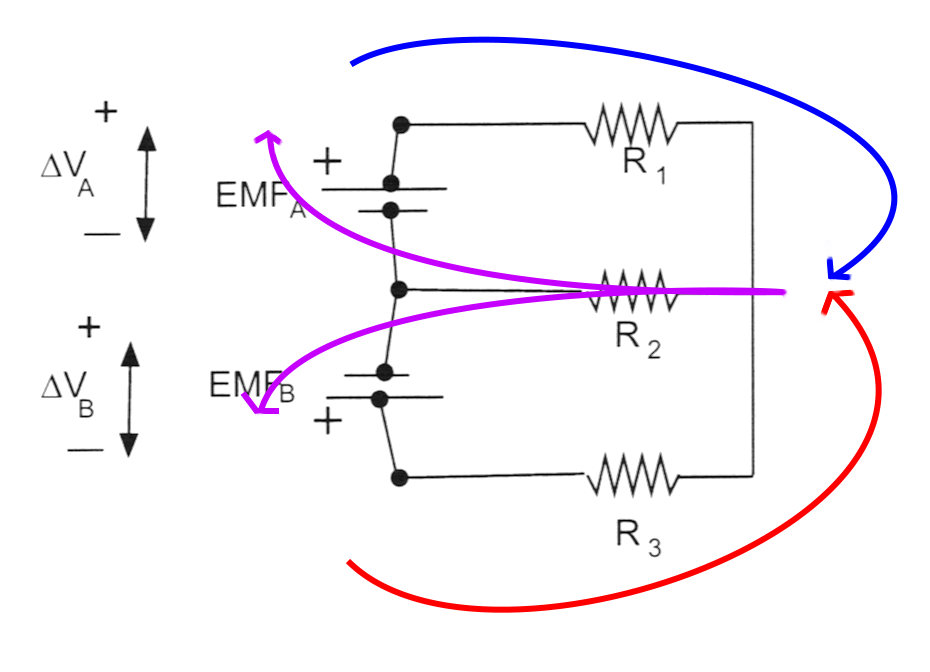
\includegraphics{phys152_lab7_circuitdiagram}\\
			
			Measured vs Calculated Plots with Error Bars \\\\
			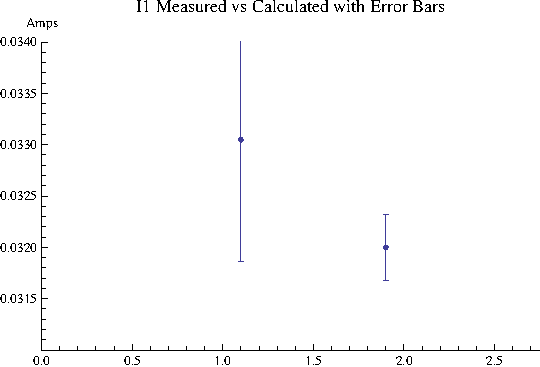
\includegraphics[width=300px]{lab7_graph1} \\
			
			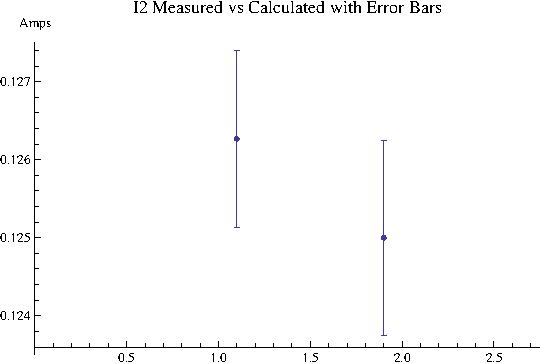
\includegraphics[width=300px]{lab7_graph2} \\
			
			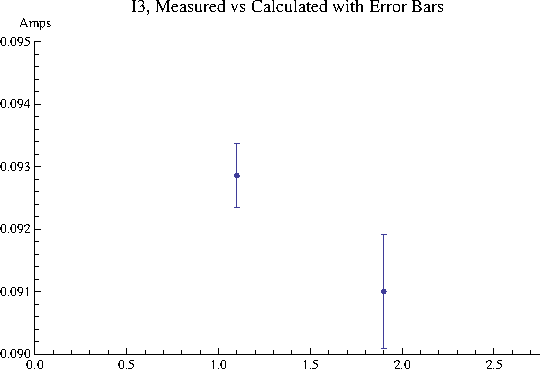
\includegraphics[width=300px]{lab7_graph3} \\
			

\endgroup
\begingroup
	\section{Uncertainty Calculations}\hfill\\
		\let\clearpage\relax
			See Data Tables section
\endgroup
\begingroup
	\section{Results}\hfill\\
		\let\clearpage\relax
			\begin{center}
\textbf{Calculated vs Measured Current} \\
\begin{tabular}{| l | l | l | l |}
	\hline
	I Branch&Calculated (A)&Measured (A)&Error \\ \hline
	1&0.0330472&0.032&0.032198  \\ \hline
	2&0.126267&0.125&0.010029 \\ \hline
	3&0.092857& 0.091&0.020200 \\ \hline
\end{tabular}

See Graphs and Diagrams for plots with error bars.

\end{center}
\endgroup
\begingroup
	\section{Discussion}\hfill\\
		\let\clearpage\relax
			
We began by assembling the circuit of three resistors and two power supplies as outlined in the lab procedure.  Both negative terminals of the power supplies were connected to a resistor ($R_2$) that was measured at 10.85 $\Omega$.  The positive terminal of power supply A connected to $R_1$ which measured 4.66 $\Omega$.  The positive terminal of power supply B connected to $R_3$ that was measured at 1.54 $\Omega$.  The unconnected sides of $R_1$ and $R_3$ were connected to the unconnected end of $R_2$.  When the power supplies were switched on, we measured the voltage across each resistor (see Data Sheet \#1 for measurements).  Using Ohm's law, we calculated the values of the current for each of the three segments of the circuit.  Finally we measured the current directly by placing the leads of the Ammeter inline between each of the two positive terminals of the batteries and the negative terminals with their respective resistors.
\endgroup
\begingroup
	\section{Questions and Answers }\hfill\\
		\let\clearpage\relax
			\begin{enumerate}[1.] %TODO
	\item Were your initial assumptions for directions of current completely correct? \\
	
	Yes, at least at the point when we came to an understanding of where the measurements for current should be taken.
	
	\item For Part E's data above, did the two different meter settings for the current measurements make any difference in the measured currents?  Why or why not?
	
	At least at the voltage from our power supplies they made an incredible amount of difference.  For example, at the 200 mA setting, the measurements for $I_1$ and $I_3$ were zero which is clearly not precise enough to use for further calculations or comparisons to other measurements.
	
\end{enumerate}
\endgroup
\end{document}